\setAuthor{Jaan Kalda}
\setRound{piirkonnavoor}
\setYear{2024}
\setNumber{G 7}
\setDifficulty{7}
\setTopic{TODO}

\prob{Palgid vees}
\begin{wrapfigure}{r}{0.3\textwidth}
  \vspace{-25pt}
  \begin{center}
  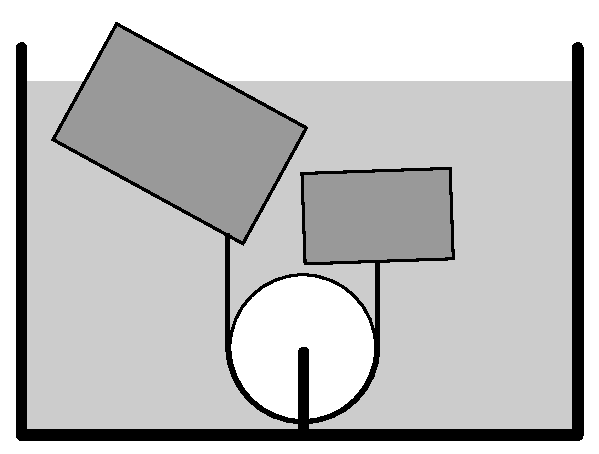
\includegraphics[scale=0.3]{2024-v2g-07-yl.pdf}
  \vspace{-20pt}
  \end{center}
\end{wrapfigure}

Kaks palki on kinnitatud üksteise külge nööri abil, mis läheb üle basseini põhja kinnitatud ploki nii nagu näidatud joonisel. Nöör on tõmmanud ühe palgi üleni vee alla sel ajal kui teine ujub vee pinnal. Mõlema palgi tihedus on $\rho=\SI {600}{\kg \per\m\cubed}$, vee tihedus $\rho_v=\SI{1000}{\kg\per\m\cubed}$, väiksema palgi ruumala on $V=\SI{30}\litre$ ja risttahuka kujulise basseini põhja pindala  $S=\SI{1}{m\squared}$. Kui palju muutub veetaseme kõrgus basseinis, kui palke ühendav nöör katki lõigata?


\hint

\solu
Süsteemile vesi+palgid mõjub raskusjõud, mille tasakaalustab jõud $pS-2T$, kus $T$ on jõud, millega niit tõmbab kumbagi palki. Idee vaadelda süsteemi vesi+palgid koos annab \p{2}; tasakaalutingimusest saadud raskusjõu avaldis $pS-2T$ annab \p{2}. Väiksema palgi tasakaalutingimusest saame, et $T=(\rho_v- \rho)Vg$ \p{1}. Kui niit katki lõigata, siis niidi pinge kaob, kuid süsteemile vesi+palgid mõjub raskusjõud jõud peab samaks jääma \p{1}. Seega rõhumisjõu muutus $S\Delta p=2T$ \p{1}. Et $\Delta p=\rho_vg\Delta h$ \p{1}, siis veetase langeb kõrguse $\delta h=2T/\rho_vgS=2(\rho_v- \rho)V/\rho_vS=\SI{2.4}{\cm}$ (valem \p{1}, arvväärtus \p{1}).

Alternatiivne lahendus.  Väiksema palgi tasakaalutingimusest saame, et $T=(\rho_v- \rho)Vg$ \p{1}. Olgu suurema palgi koguruumala $U$, millest vee all on ruumala $W$. Sellisel juhul saame selle tasakaalutingimuseks $\rho_v Wg= \rho Ug+T$ \p{1}. Kahest avaldisest saame kokku $W=kU+V-kV$ \p{1}, kus $k=\rho/\rho_v$. Kui nöör on katki, siis on palkide veealuste osade ruumalad tasakaalutingimusest tulenevalt vastavalt $Vk$ ja $Uk$ (\p{1+1}). Enne oli palkide veealuste osade ruumalade summa $W+V$ \p{1} ja pärast --- $Vk+Uk$ \p{1}, seega veealuste osade ruumala vähenes $W+V-Vk-Uk=2V(1-k)$ võrra \p{1}, mistõttu alanes veetase $2V(1-k)/S=\SI{2.4}{\cm}$ võrra (valem \p{1}, arvväärtus \p{1}).
\probend